\documentclass[conference]{IEEEtran}
\IEEEoverridecommandlockouts
% The preceding line is only needed to identify funding in the first footnote. If that is unneeded, please comment it out.
\usepackage{cite}
\usepackage{amsmath,amssymb,amsfonts}
\usepackage{algorithmic}
\usepackage{graphicx}
\usepackage{textcomp}
\usepackage{xcolor}
\usepackage{subfig}
\usepackage{float}

\def\BibTeX{{\rm B\kern-.05em{\sc i\kern-.025em b}\kern-.08em
    T\kern-.1667em\lower.7ex\hbox{E}\kern-.125emX}}
\begin{document}

\title{MO443 - Assignment II}

\author{210404 -- Guilherme Vieira Leite}

\maketitle

\section{Introduction}
Dithering, or half-tone, is widely used to reduce the amount of data that travels through a medium, as in television signal being transmitted through airwaves to newspaper printing in only black and white. In this work, we explore the implementation of some dithering variants with error diffusion and their effects on the input image.\par
This work is structured as such: Section~\ref{sec:method} explains our method, and which aspects of dithering we will explore in the following section, and our input images. Our results are presented in Section~\ref{sec:results}, in which we compare the methods against each other and discuss their results. Section~\ref{sec:conclusion} concludes this work with some consideration regarding our findings, and a future work direction to follow. Finally Section~\ref{sec:appendix1} acts as an Appendix to our matrices that were better stored separately from the main body.
\section{Dithering Methods}
\label{sec:method}
The implemented dithering methods in this work differentiates between each other by a couple of factors: (i) whether they are grayscaled or colored, and (ii) the error diffusion matrix.
\paragraph{Color space} Dithering in the grayscale color space is performed as in the algorithm discussed in class, in a few words: the pixel is binarized, its error is calculated and multiplied by the mask value relative to that pixel. To transfer this process to the RGB color space, we treated each of its three bands as if they were separate grayscale images, that were later combined to create a dithered colored image.
\paragraph{Filter matrix} Each pixel is dithered by an error metric to its neighborhood, this neighborhood is defined by the filter matrix, how large it is and which pixels are considered in the metric. In this work, we tested on six pre-defined error diffusion matrices: Floyd and Steinberg, Stevenson and Arce, Burkes, Sierra, Stucki, and Jarvis, Judice, and Ninke, seen in Section~\ref{sec:appendix1}.
\section{Experiments}
Throughout our experiments, we aimed to explore the effects of dithering, while varying the color space, the error diffusion matrix and the order in which the error was diffused. We also exchanged the output's quality by lower processing time, shrinking all input images to around 128x128, but the algorithm is still able to process larger images.\par
We performed dithering on nine images, some provided by the professor and some particularly obtained. The images were chosen to exhaust the algorithm and explore their weaknesses and strengths, especially the colored dithering. Figure~\ref{fig:input} presents a few samples of the chosen images.
\begin{figure}[htbp]
\centering
\subfloat{
	{
		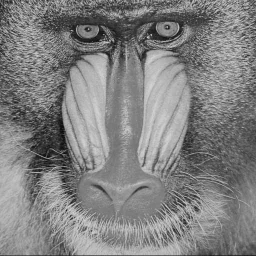
\includegraphics[scale=0.35]{figures/input/baboon}
	}
	\label{fig:baboon}
}
\subfloat{
	{
		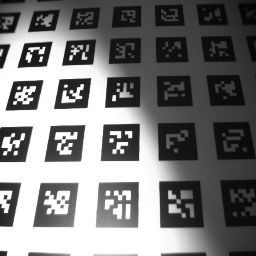
\includegraphics[scale=0.35]{figures/input/fiducial}
	}
	\label{fig:bee}
}
\quad
\subfloat{
	{
		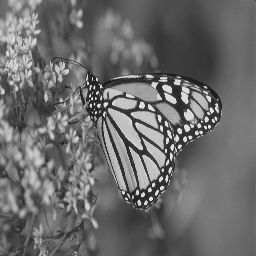
\includegraphics[scale=0.35]{figures/input/monarch}
	}
	\label{fig:juquinha}
}
\subfloat{
	{
		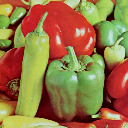
\includegraphics[scale=0.35]{figures/input/peppers}
	}
	\label{fig:peppers}
}
\quad
\subfloat{
	{
		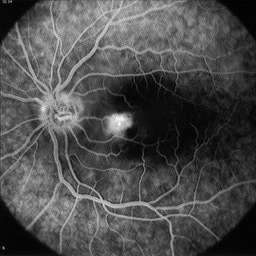
\includegraphics[scale=0.35]{figures/input/retina}
	}
	\label{fig:sky}
}
\subfloat{
	{
		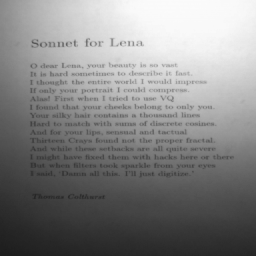
\includegraphics[scale=0.35]{figures/input/sonnet}
	}
	\label{fig:tattoo}
}
\caption{A sample of the images used in the experiments.}
\label{fig:input}
\end{figure}\par

\begin{figure}[htbp]
\centering
\subfloat{
	{
		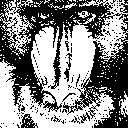
\includegraphics[scale=0.7]{figures/global/global_128_baboon.png}
	}
	\label{fig:baboon}
}
\subfloat{
	{
		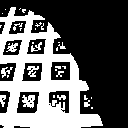
\includegraphics[scale=0.7]{figures/global/global_128_fiducial.png}
	}
	\label{fig:bee}
}
\quad
\subfloat{
	{
		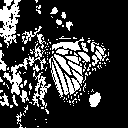
\includegraphics[scale=0.7]{figures/global/global_128_monarch.png}
	}
	\label{fig:juquinha}
}
\subfloat{
	{
		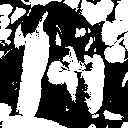
\includegraphics[scale=0.7]{figures/global/global_128_peppers.png}
	}
	\label{fig:peppers}
}
\quad
\subfloat{
	{
		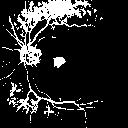
\includegraphics[scale=0.7]{figures/global/global_128_retina.png}
	}
	\label{fig:sky}
}
\subfloat{
	{
		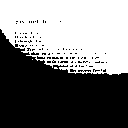
\includegraphics[scale=0.7]{figures/global/global_128_sonnet.png}
	}
	\label{fig:tattoo}
}
\caption{A sample of the images used in the experiments.}
\label{fig:input}
\end{figure}\par

We also experimented with three traversal methods, looping through the image from (i) left to right, top to bottom, (ii) right to left, bottom to top, and (iii) top to bottom, but every even row was looped left to right and every odd row was looped from right to left, seen in Figure~\ref{fig:traversal}. To traverse the images in these varying methods a few precautions had to be taken since the chosen filters generate a particular effect, in which any pixel already dithered will be ignored to future error diffusion. We need to accommodate this effect on any traversal that differs from left to right, top to bottom, and we did so by tweaking with the filter's matrix to match the expected result, one example on Floyd and Steinberg can be seen in Table~\ref{tab:flo_inverse}.
\begin{figure}[htbp]
	\centering
	\subfloat{
		{
			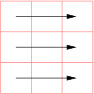
\includegraphics[scale=0.5]{figures/l2r}
		}
		\label{fig:l2r}
	}
	\quad
	\subfloat{
		{
			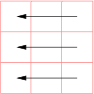
\includegraphics[scale=0.5]{figures/r2l}
		}
		\label{fig:r2l}
	}
	\quad
	\subfloat{
		{
			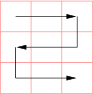
\includegraphics[scale=0.5]{figures/zz}
		}
		\label{fig:zz}
	}
	\caption{Traversal directions experimented on.}
	\label{fig:traversal}
\end{figure}
\begin{table}[!h]
\centering
\renewcommand{\arraystretch}{1.5}
\begin{tabular}{c|c|c}
1/16 & 5/16             & 3/16 \\ \hline
7/16 & \textit{f(x, y)} &     
\end{tabular}
\caption{Floyd and Steinberg's diffusion error matrix when traversing from right to left, bottom to right.}
\label{tab:flo_inverse}
\end{table}
\section{Results}
\label{sec:results}
In this section, we present and discuss the results obtained from the methods discussed in Section~\ref{sec:method}. To better explore the different aspects of a dithering process we focus our discussion on three subsections bellow.
\subsection{Color space}
In this experiment, we performed a colored dithering and a grayscaled one. Although we are not exploring the effects of error diffusion and traversal direction, we also used Floyd and Steinberg's error diffusion and traversed the image from left to right, top to bottom. Figure~\ref{fig:baboon_colorspace} shows the resulting dithering, in it we can observe that overall features of the image are kept, it is still possible to identify the baboon in Figure~\ref{fig:baboon_color}, as it is the intention of dithering. But on a closer inspection it is also possible to notice a drop in quality of both images, also an expected effect, for instance, the lower lip of the baboon has been filled with noise and mixes with the fur, another side effect of dithering is the loss of small details, as seen in Figure~\ref{fig:sky_color} the skylines at the distance are almost indiscernible.
\begin{figure}[htbp]
	\centering
	\subfloat[Color baboon]{
		{
			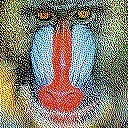
\includegraphics[scale=0.7]{figures/left2right/flo_color_baboon}
		}
		\label{fig:baboon_color}
	}
	\subfloat[Gray baboon]{
		{
			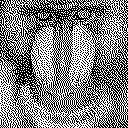
\includegraphics[scale=0.7]{figures/left2right/flo_gray_baboon}
		}
		\label{fig:baboon_gray}
	}
	\quad
	\subfloat[Color sky]{
		{
			\includegraphics[scale=0.7]{figures/left2right/flo_color_sky}
		}
		\label{fig:sky_color}
	}
	\subfloat[Gray sky]{
		{
			\includegraphics[scale=0.7]{figures/left2right/flo_gray_sky}
		}
		\label{fig:sky_gray}
	}
	\caption{Color and Grayscale dithering.}
	\label{fig:baboon_colorspace}
\end{figure}
\subsection{Dithering matrices}
\label{ssec:matrix}
In this experiment, we investigated the effects of a pixel's neighborhood in dithering. We generated the same dithered image for each of the six masks presented in Section~\ref{sec:method}, both in color and grayscale, Figures~\ref{fig:color_error_diffusion} and~\ref{fig:gray_error_diffusion}, and as in the previous experiment, we fixed the traverse direction from left to right, top to bottom.
\begin{figure}[htbp]
	\centering
	\subfloat[Floyd \& Steinnberg]{
		{
			\includegraphics[scale=0.7]{figures/left2right/flo_color_tattoo}
		}
		\label{fig:flo_color_tattoo}
	}
	\subfloat[Stevenson \& Arce]{
		{
			\includegraphics[scale=0.7]{figures/left2right/ste_color_tattoo}
		}
		\label{fig:ste_color_tattoo}
	}
    \quad
	\subfloat[Burkes]{
		{
			\includegraphics[scale=0.7]{figures/left2right/bur_color_tattoo}
		}
		\label{fig:bur_color_tattoo}
	}
	\subfloat[Sierra]{
		{
			\includegraphics[scale=0.7]{figures/left2right/sie_color_tattoo}
		}
		\label{fig:sie_color_tattoo}
	}\quad
	\subfloat[Stucki]{
		{
			\includegraphics[scale=0.7]{figures/left2right/stu_color_tattoo}
		}
		\label{fig:stu_color_tattoo}
	}
	\subfloat[Jarvis, Judice, \& Ninke]{
		{
			\includegraphics[scale=0.7]{figures/left2right/jar_color_tattoo}
		}
		\label{fig:jar_color_tattoo}
	}
	\caption{Color error diffusion on Tattoo.}
	\label{fig:color_error_diffusion}
\end{figure}\par
The results with colored images are shown in Figure~\ref{fig:color_error_diffusion}, and it is possible to notice that the biggest difference resides between Fig~\ref{fig:ste_color_tattoo} and the rest. In Stevenson and Arce's method, a lot of the noise was increased, creating thicker borders but also disrupting the color of the skin with pink and green pixels. It is also interesting to notice that the methods of Sierra Fig.~\ref{fig:sie_color_tattoo}, Stucki Fig.~\ref{fig:stu_color_tattoo}, and Jarvis et al. Fig.~\ref{fig:jar_color_tattoo} improved the borders of the original image, Figure~\ref{fig:tattoo}, especially in the bee black and yellow stripes which were blurred.
\begin{figure}[htbp]
	\centering
	\subfloat[Floyd \& Steinnberg]{
		{
			\includegraphics[scale=0.7]{figures/left2right/flo_gray_tattoo}
		}
		\label{fig:flo_gray_tattoo}
	}
	\subfloat[Stevenson \& Arce]{
		{
			\includegraphics[scale=0.7]{figures/left2right/ste_gray_tattoo}
		}
		\label{fig:ste_cgray_tattoo}
	}
    \quad
	\subfloat[Burkes]{
		{
			\includegraphics[scale=0.7]{figures/left2right/bur_gray_tattoo}
		}
		\label{fig:bur_gray_tattoo}
	}
	\subfloat[Sierra]{
		{
			\includegraphics[scale=0.7]{figures/left2right/sie_gray_tattoo}
		}
		\label{fig:sie_gray_tattoo}
	}
	\quad
	\subfloat[Stucki]{
		{
			\includegraphics[scale=0.7]{figures/left2right/stu_gray_tattoo}
		}
		\label{fig:stu_gray_tattoo}
	}
	\subfloat[Jarvis, Judice, \& Ninke]{
		{
			\includegraphics[scale=0.7]{figures/left2right/jar_gray_tattoo}
		}
		\label{fig:jar_gray_tattoo}
	}
	\caption{Grayscale error diffusion on Tattoo.}
	\label{fig:gray_error_diffusion}
\end{figure}\par
There are not many differences between the color and grayscale masks applications, but in Figure~\ref{fig:gray_error_diffusion} it is even easier to spot the noise effect caused by Stevenson and Arce's mask. Most of the bee's wings also vanished in the background, but that is a side effect of the grayscale transform process and not the application of the masks.
\subsection{Traversal directions}
In this experiment we test three traversal directions and discuss their effect on the output image, the experiment was performed on Figure~\ref{fig:bee}, using Floyd and Steinberg's mask, its colored result is shown in Figure~\ref{fig:color_traversal} and the grayscaled output in Figure~\ref{fig:gray_traversal}.
\begin{figure}[htbp]
	\centering
	\subfloat[Left to right]{
		{
			\includegraphics[scale=0.8]{figures/left2right/flo_color_bee}
		}
		\label{fig:l2r_flo_color_bee}
	}
	\quad
	\subfloat[Right to left]{
		{
			\includegraphics[scale=0.8]{figures/right2left/flo_color_bee}
		}
		\label{fig:r2l_flo_color_bee}
	}
	\subfloat[Zig zag]{
		{
			\includegraphics[scale=0.8]{figures/zigzag/flo_color_bee}
		}
		\label{fig:zz_flo_color_bee}
	}
	\caption{Color traversal direction on Girl.}
	\label{fig:color_traversal}
\end{figure}
In Figure~\ref{fig:l2r_flo_color_bee} we traversed the image from left to right, top to bottom, and in Figure~\ref{fig:r2l_flo_color_bee} from right to left, bottom to top. These outputs differ from one another on subtle ways, for example the girl's lips in Figure~\ref{fig:l2r_flo_color_bee} looks serious, as in the original Figure~\ref{fig:bee}, but in Figure~\ref{fig:r2l_flo_color_bee} they were extended and form a subtle smile, other than this detail we can notice a few differences in the white background at the top where it forms a wavy pattern in Figure~\ref{fig:l2r_flo_color_bee} and diagonal patterns in Figure~\ref{fig:r2l_flo_color_bee}. The third approach or the zig zag traversal, show in Figure~\ref{fig:zz_flo_color_bee}, disrupted the image by introducing a great amount of noise, and similarly to Figure~\ref{fig:l2r_flo_color_bee} a wavy pattern at the top.
\begin{figure}[htbp]
	\centering
	\subfloat[Left to right]{
		{
			\includegraphics[scale=0.8]{figures/left2right/flo_gray_bee}
		}
		\label{fig:l2r_flo_gray_bee}
	}
	\quad
	\subfloat[Right to left]{
		{
			\includegraphics[scale=0.8]{figures/right2left/flo_gray_bee}
		}
		\label{fig:r2l_flo_gray_bee}
	}
	\subfloat[Zig zag]{
		{
			\includegraphics[scale=0.8]{figures/zigzag/flo_gray_bee}
		}
		\label{fig:zz_flo_gray_bee}
	}
	\caption{Grayscale traversal direction on Girl.}
	\label{fig:gray_traversal}
\end{figure}
The grayscale images shown in Figure~\ref{fig:gray_traversal} illustrates similar problems as the ones from Section~\ref{ssec:matrix}, the images gets more blurry due to color loss and the noise seen in Figure~\ref{fig:zz_flo_color_bee} is also seen in Figure~\ref{fig:zz_flo_gray_bee}.
\subsection{Error function}
In this section we want to discuss an experiment that we performed \textit{accidentally} by committing a mistake in the error function calculation. Upon performing the error calculation we overflowed its maximum value, which turned roughly every other pixel into a black one. The output can be seen in Figure~\ref{fig:error}, it is similar to the desired result, except a lot darker due to the abundance of black pixels.
\begin{figure}[htbp]
	\centering
	\subfloat[Desired]{
		{
			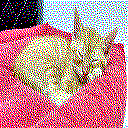
\includegraphics[scale=0.8]{figures/left2right/flo_color_juquinha}
		}
		\label{fig:juquinha2}
	}
	\subfloat[Error]{
		{
			\includegraphics[scale=0.2]{figures/error}
		}
		\label{fig:error1}
	}
	\caption{Mistake in error function generated a darker image.}
	\label{fig:error}
\end{figure}
\section{Conclusions}
This work proposed to explore a few aspects of dithering with error diffusion, we went through the differences regarding the color space, the neighborhood relevance, and the direction to loop the input. Overall only a few masks produced an inferior result than expected, and in our experiments, the \textit{zig zag} traversal performed as worst among its alternatives. As future work, the exploration of a diagonal traversal should be considered.
\pagebreak
\section{Appendix I}
\label{sec:appendix1}

\begin{table}[!h]
\centering
\renewcommand{\arraystretch}{1.5}
\begin{tabular}{c|c|c}
     & \textit{f(x, y)} & 7/16 \\ \hline
3/16 & 5/16             & 1/16
\end{tabular}
\caption{Floyd and Steinberg's diffusion error matrix.}
\label{tab:flo}
\end{table}

\begin{table}[!h]
\centering
\renewcommand{\arraystretch}{1.5}
\begin{tabular}{c|c|c|c|c|c|c}
 & \textit{} &  & \textit{f(x, y)} &  & 32/200 &  \\ \hline
12/200 &  & 26/200 &  & 30/200 &  & 16/200 \\ \hline
 & 12/200 &  & 26/200 &  & 12/200 &  \\ \hline
5/200 &  & 12/200 &  & 12/200 &  & 5/200
\end{tabular}
\caption{Stevenson and Arce's diffusion error matrix.}
\label{tab:ste}
\end{table}

\begin{table}[!h]
\centering
\renewcommand{\arraystretch}{1.5}
\begin{tabular}{c|c|c|c|c}
 &  & \textit{f(x, y)} & 8/32 & 4/32 \\ \hline
2/32 & 4/32 & 8/32 & 4/32 & 2/32
\end{tabular}
\caption{Burkes' diffusion error matrix.}
\label{tab:bur}
\end{table}

\begin{table}[!h]
\centering
\renewcommand{\arraystretch}{1.5}
\begin{tabular}{c|c|c|c|c}
 &  & \textit{f(x, y)} & 5/32 & 3/32 \\ \hline
2/32 & 4/32 & 5/32 & 4/32 & 2/32 \\ \hline
 & 2/32 & 3/32 & 2/32 & 
\end{tabular}
\caption{Sierra's diffusion error matrix.}
\label{tab:sie}
\end{table}

\begin{table}[!h]
\centering
\renewcommand{\arraystretch}{1.5}
\begin{tabular}{l|l|l|l|l}
 &  & \textit{f(x, y)} & 8/42 & 4/42 \\ \hline
2/42 & 4/42 & 8/42 & 4/42 & 2/42 \\ \hline
1/42 & 2/42 & 4/42 & 2/42 & 1/42
\end{tabular}
\caption{Stucki's diffusion error matrix.}
\label{tab:stu}
\end{table}

\begin{table}[!h]
\centering
\renewcommand{\arraystretch}{1.5}
\begin{tabular}{l|l|l|l|l}
 &  & \textit{f(x, y)} & 7/48 & 5/48 \\ \hline
3/48 & 5/48 & 7/48 & 5/48 & 3/48 \\ \hline
1/48 & 3/48 & 5/48 & 3/48 & 1/48
\end{tabular}
\caption{Jarvis, Judice, and Ninke's diffusion error matrix.}
\label{tab:jar}
\end{table}

\end{document}
